\documentclass[xetex,mathserif,serif]{beamer}
\usepackage{polyglossia}
\setdefaultlanguage[babelshorthands=true]{russian}
\usepackage{minted}
\usepackage{tabu}

\useoutertheme{infolines}

\usepackage{fontspec}
\setmainfont{FreeSans}
\newfontfamily{\russianfonttt}{FreeSans}

\definecolor{links}{HTML}{2A1B81}
\hypersetup{colorlinks,linkcolor=,urlcolor=links}

\tabulinesep=0.7mm

\newcommand{\attribution}[1] {
    \vspace{-5mm}\begin{flushright}\begin{scriptsize}\textcolor{gray}{\textcopyright\, #1}\end{scriptsize}\end{flushright}
}

\title{Практика 8: Развёртывание, Docker}
\author[Юрий Литвинов]{Юрий Литвинов \newline
    \textcolor{gray}{\small\texttt{yurii.litvinov@gmail.com}} \newline
    \textcolor{gray}{\small Спасибо \textcolor{black}{Владиславу Танкову} (\texttt{vdtankov@gmail.com}) за  предоставленные материалы}
}

\date{26.05.2020г}

\begin{document}

    \frame{\titlepage}

    \section{Введение}

    \begin{frame}
        \frametitle{CI и CD}
        \begin{itemize}
            \item Проекты разрабатываются большими командами
            \begin{itemize}
                \item Разработчики
                \item Тестировщики
                \item Администраторы
            \end{itemize}
            \item Разное окружение, разные форматы, разная история изменений
            \item Нужен артефакт, инкапсулирующий в себе окружение и приложение
            \begin{itemize}
                \item Легко создавать и передавать
                \item Не влияет на производительность
            \end{itemize}
        \end{itemize}
    \end{frame}

    \begin{frame}
        \frametitle{Docker}
        \begin{itemize}
            \item Средство для ``упаковки'' приложений в изолированные контейнеры
            \item Что-то вроде легковесной виртуальной машины
            \item Широкий инструментарий: DSL для описания образов, публичный репозиторий, поддержка оркестраторами
        \end{itemize}
        \begin{center}
            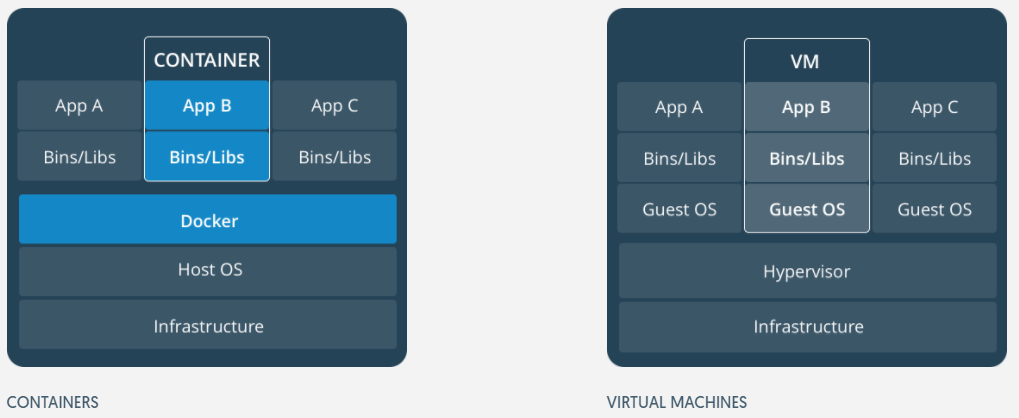
\includegraphics[width=0.7\textwidth]{docker.png}
            \attribution{\url{https://www.docker.com}}
        \end{center}
    \end{frame}

    \begin{frame}
        \frametitle{Чем он помогает}
        \begin{center}
            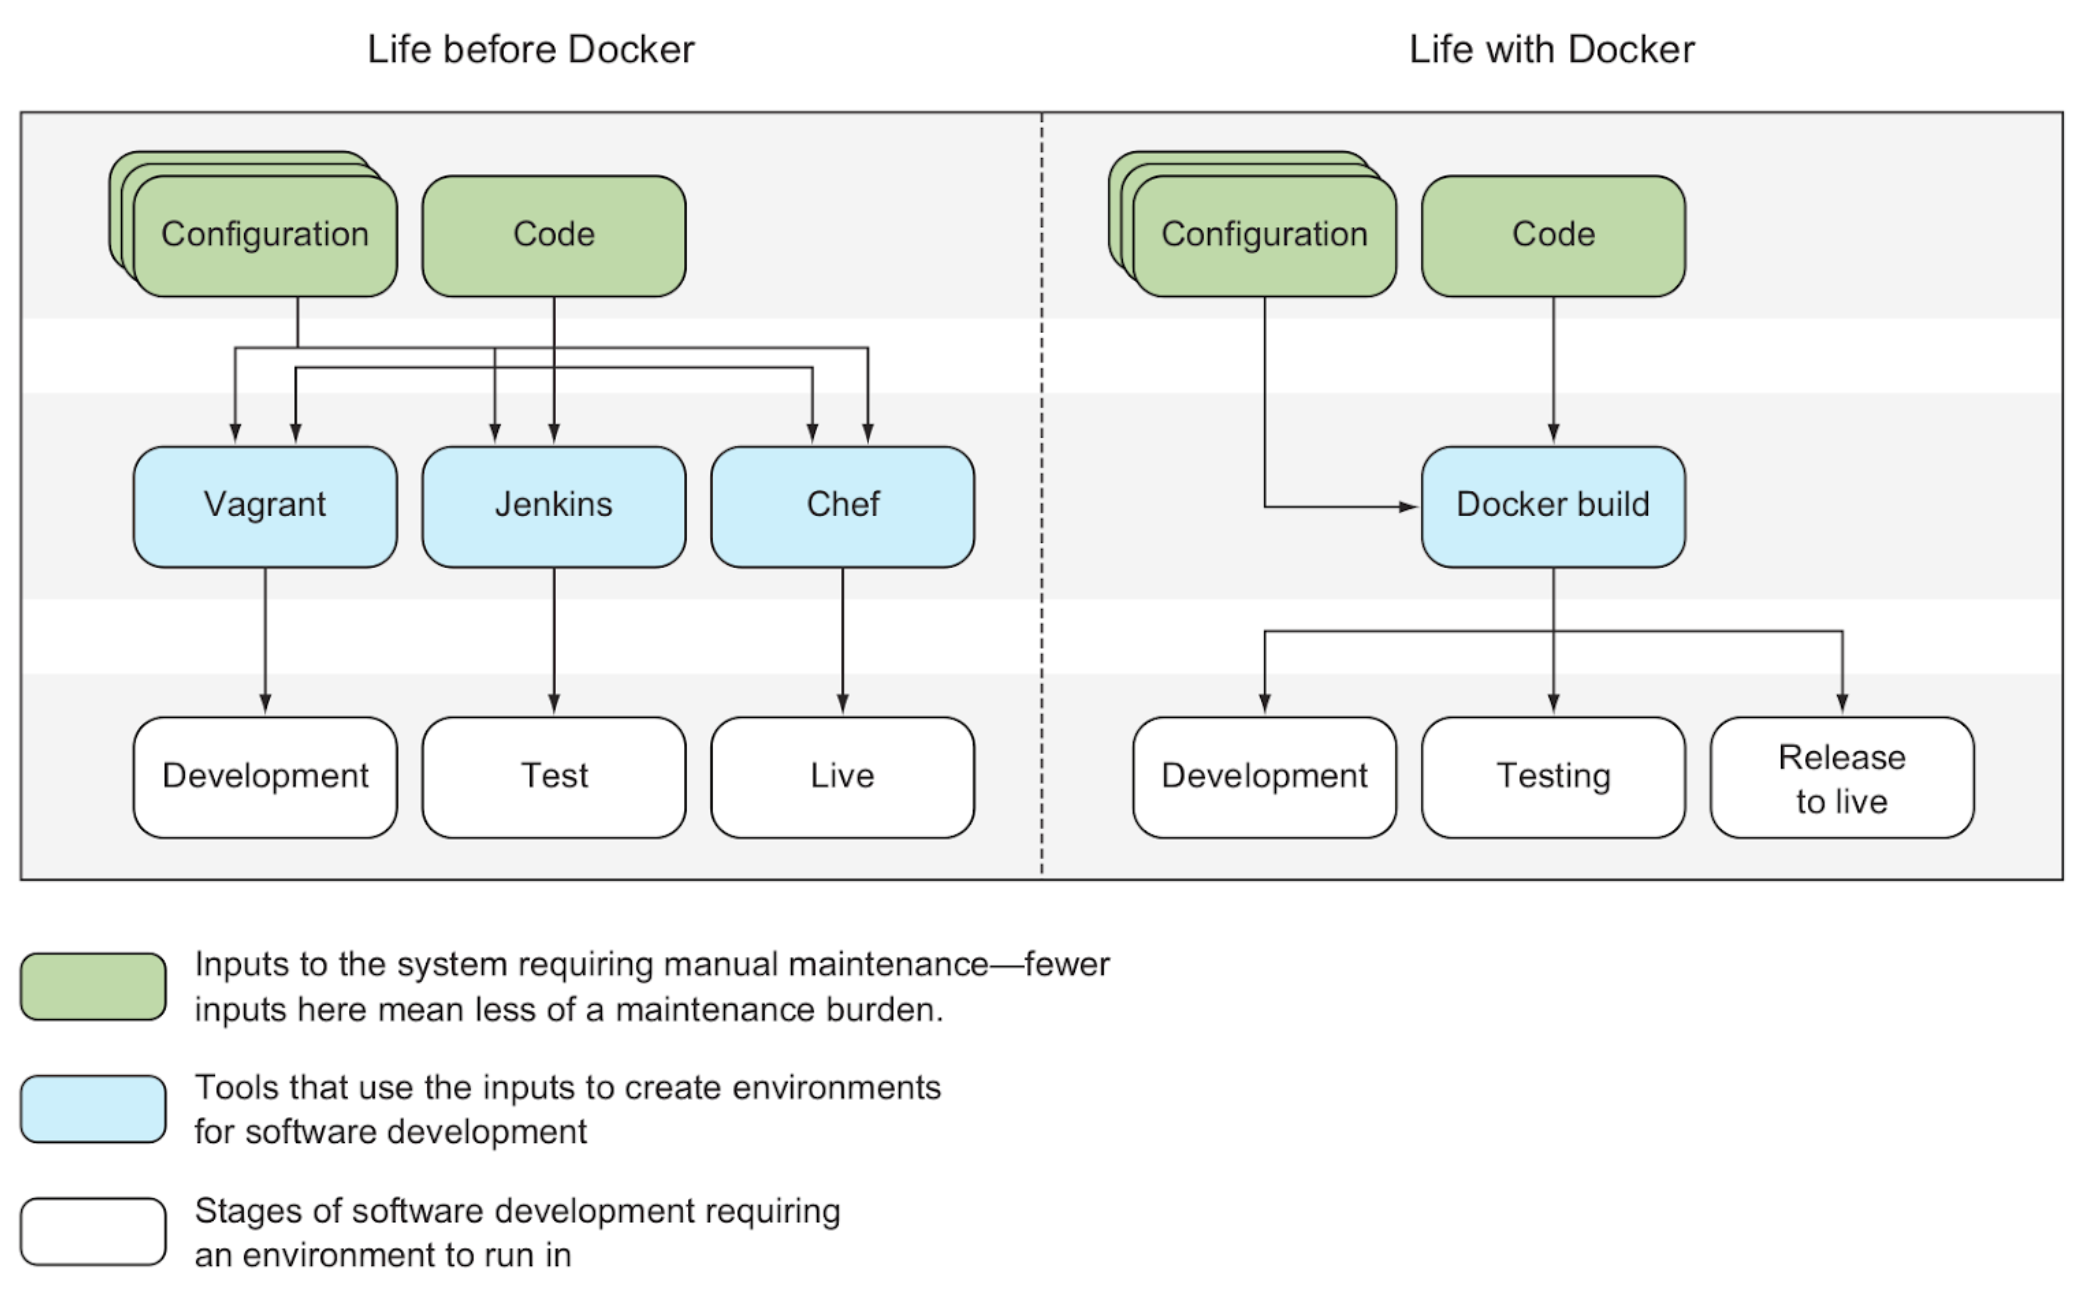
\includegraphics[width=0.9\textwidth]{withAndWithoutDocker.png}
        \end{center}
    \end{frame}

    \section{Архитектура Docker}

    \begin{frame}
        \frametitle{Docker Image}
        \begin{columns}
            \begin{column}{0.6\textwidth}
                \begin{itemize}
                    \item Окружение и приложение
                    \item Состоит из слоёв
                    \begin{itemize}
                        \item Все слои read-only
                        \item Образы делят слои между собой как процессы делят динамические библиотеки
                    \end{itemize}
                    \item На основе одного образа можно создать другой
                \end{itemize}
            \end{column}
            \begin{column}{0.4\textwidth}
                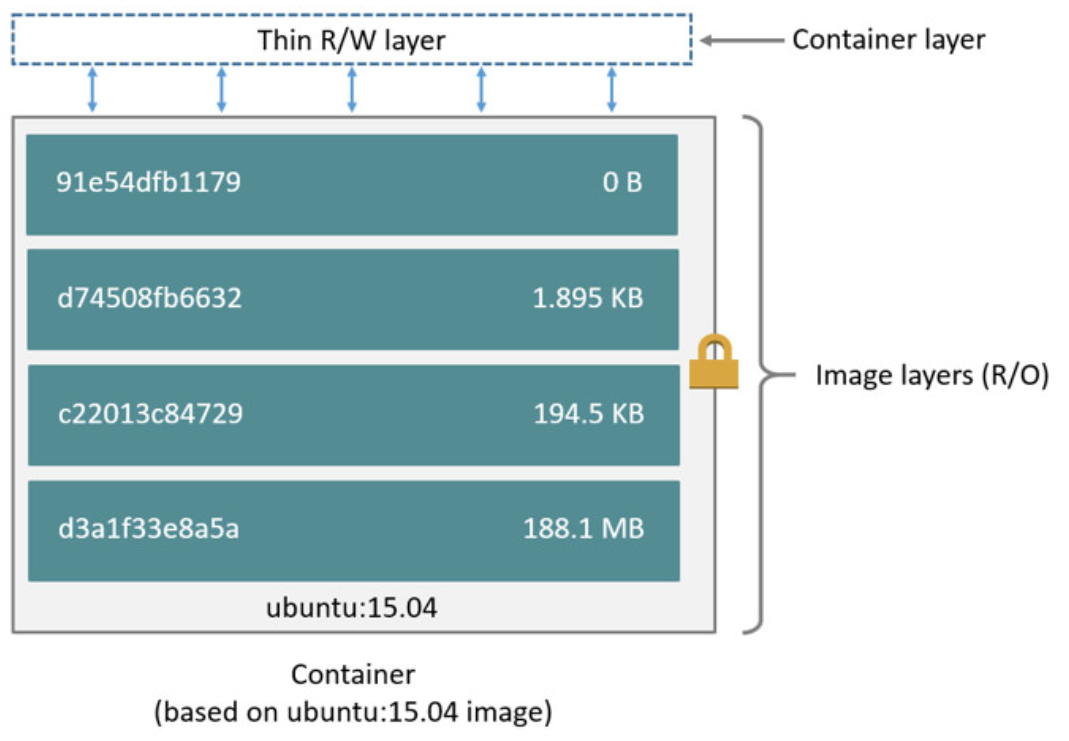
\includegraphics[width=0.9\textwidth]{dockerLayers.png}
            \end{column}
        \end{columns}
    \end{frame}
    
    \begin{frame}
        \frametitle{Docker Container}
        \begin{columns}
            \begin{column}{0.5\textwidth}
                \begin{itemize}
                    \item Образ с дополнительным write слоем
                    \item Содержит один запущенный процесс
                    \item Может быть сохранен как новый образ
                \end{itemize}
            \end{column}
            \begin{column}{0.5\textwidth}
                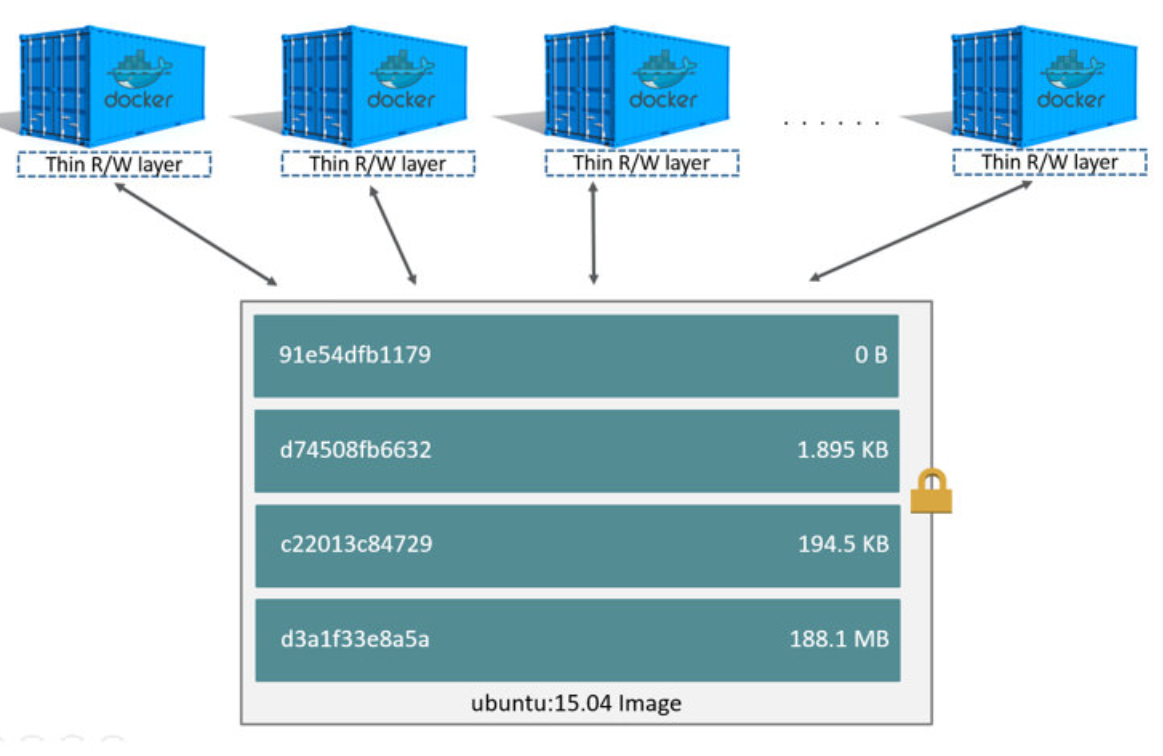
\includegraphics[width=0.9\textwidth]{dockerContainer.png}
            \end{column}
        \end{columns}
    \end{frame}

    \begin{frame}
        \frametitle{Клиент и сервер}
        \begin{itemize}
            \item Docker --- это клиент-серверное приложение
            \item Docker Daemon
            \begin{itemize}
                \item REST API
                \item Управляет запущенными контейнерами
                \item Управляет локальным репозиторием образов
            \end{itemize}
            \item Docker Client
            \begin{itemize}
                \item CLI для Docker
                \item Запросы по HTTP пересылает Docker Daemon
            \end{itemize}
        \end{itemize}
    \end{frame}

    \begin{frame}
        \frametitle{DockerHub}
        \begin{columns}
            \begin{column}{0.5\textwidth}
                \begin{itemize}
                    \item Внешний репозиторий образов
                    \begin{itemize}
                        \item Официальные образы
                        \item Пользовательские образы
                        \item Приватные репозитории
                    \end{itemize}
                    \item Простой CI/CD
                    \item Высокая доступность
                \end{itemize}
            \end{column}
            \begin{column}{0.5\textwidth}
                
\includegraphics[width=0.9\textwidth]{dockerHub.png}
            \end{column}
        \end{columns}
    \end{frame}

    \section{Как этим пользоваться}

    \begin{frame}
        \frametitle{Базовые команды}
        \begin{itemize}
            \item docker run --- запускает контейнер (при необходимости делает pull)
            \begin{itemize}
                \item -d --- запустить в фоновом режиме
                \item -p host\_port:container\_port --- прокинуть порт из контейнера на хост
                \item -i -t --- запустить в интерактивном режиме
                \item Пример: \mintinline{text}|docker run -it ubuntu /bin/bash|
            \end{itemize}
            \item docker ps --- показывает запущенные контейнеры
            \begin{itemize}
                \item Пример: \mintinline{text}|docker run -d nginx; docker ps|
            \end{itemize}
            \item docker stop --- останавливает контейнер (шлёт SIGTERM, затем SIGKILL)
            \item docker exec --- запускает дополнительный процесс в контейнере
        \end{itemize}
    \end{frame}

    \begin{frame}[fragile]
        \frametitle{Dockerfile}
        \begin{scriptsize}
            \begin{minted}{docker}
# Use an official Python runtime as a parent image
FROM python:2.7-slim

# Set the working directory to /app
WORKDIR /app

# Copy the current directory contents into the container at /app
ADD . /app

# Install any needed packages specified in requirements.txt
RUN pip install --trusted-host pypi.python.org -r requirements.txt

# Make port 80 available to the world outside this container
EXPOSE 80

# Define environment variable
ENV NAME World

# Run app.py when the container launches
CMD ["python", "app.py"]
            \end{minted}
        \end{scriptsize}
    \end{frame}

    \begin{frame}
        \frametitle{Команды}
        \begin{itemize}
            \item FROM --- взять как начальный образ указанный
            \item WORKDIR --- выбрать папку в качестве текущей
            \item RUN --- выполнить команду
            \item ADD --- копировать файл/папку/архив
            \item ENV --- установить environment переменную
            \item ENTRYPOINT --- установить команду для запуска процесса
            \item CMD --- установить принятые по умолчанию аргументы
            \item EXPOSE --- разрешить доступ к контейнеру по порту
            \item VOLUME --- определить mount point для volume
            \item ARG --- build аргументы
        \end{itemize}
    \end{frame}

    \begin{frame}[fragile]
        \frametitle{Пример: Redis}
        \begin{scriptsize}
            \begin{minted}{docker}
FROM ubuntu:16.04

# Install Redis.
RUN <wget ...>\
<.......>\
<.......>

# Define mountable directories.
VOLUME ["/data"]
# Define working directory.
WORKDIR /data
# Define default command.
CMD ["redis-server", "/etc/redis/redis.conf"]
# Expose ports.
EXPOSE 6379
            \end{minted}
        \end{scriptsize}
    \end{frame}

    \section{Балансировка нагрузки}

    \begin{frame}[fragile]
        \frametitle{Балансировка нагрузки}
        \framesubtitle{docker-compose.yml}
        \begin{scriptsize}
            \begin{minted}{yaml}
version: "3"
services:
    web:
        # replace username/repo:tag with your name and image details
        image: username/repo:tag
        deploy:
            replicas: 5
            resources:
                limits:
                    cpus: "0.1"
                    memory: 50M
            restart_policy:
                condition: on-failure
        ports:
            - "80:80"
        networks:
            - webnet
networks:
    webnet:
            \end{minted}
        \end{scriptsize}
    \end{frame}

    \begin{frame}
        \frametitle{Swarm-ы}
        \begin{itemize}
            \item Машина, на которой запускается контейнер, становится главной
            \item Другие машины могут присоединяться к swarm-у и получать копию контейнера
            \item Docker балансирует нагрузку по машинам
        \end{itemize}
        \begin{center}
            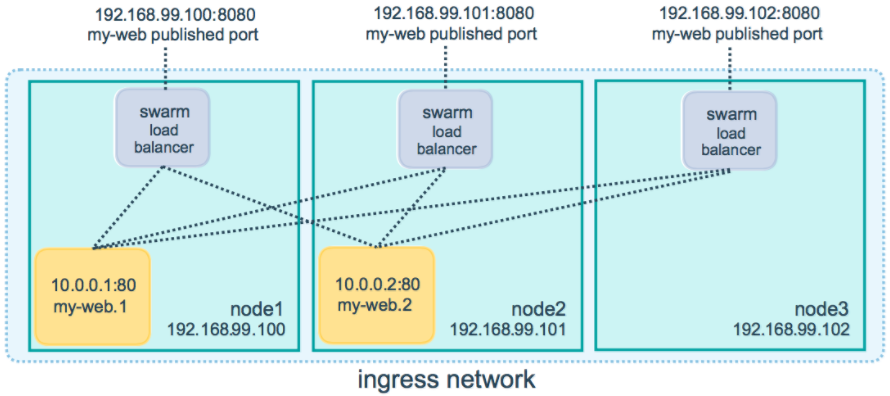
\includegraphics[width=0.7\textwidth]{swarmLoadBalancing.png}
            \attribution{\url{https://www.docker.com}}
        \end{center}
    \end{frame}

    \section{Задача}

    \begin{frame}
        \frametitle{Задание на пару}
        В командах по два человека оформить сетевой чат, разработанный на предыдущем занятии, в виде Docker-контейнера
        \begin{itemize}
            \item Убедиться, что при запуске клиента и сервера через Docker они могут установить соединение
            \item Выложить в свой репозиторий Docker-файл
        \end{itemize}
    \end{frame}

    \begin{frame}
        \frametitle{Что делать}
        \begin{itemize}
            \item Заполнить форму \url{https://forms.gle/fTaEJ2YQaBHUNmnZ6} ссылкой на репозиторий
            \item Выложить на HwProj результаты к концу пары
            \item Желательно успеть показать, что всё работает
            \item Доделать ``дома'', если не успели
        \end{itemize}
    \end{frame}

\end{document}